\documentclass[12pt]{article}
%\usepackage{float}          % необходимо для указания места картинки на странице
%\documentclass{matmex-diploma}

% русский язык:
\usepackage{polyglossia}
\setdefaultlanguage{russian}
\usepackage{fontspec}
\setmainfont[Mapping=tex-text]{CMU Serif}

% полуторный интервал:
\usepackage[nodisplayskipstretch]{setspace}
\onehalfspacing

% размеры полей
\usepackage[left=2cm,right=2cm,
    top=2cm,bottom=2cm,bindingoffset=0cm]{geometry}

%% Отступ в первом абзаце
\usepackage{indentfirst}
%% Гиперссылки
\usepackage[colorlinks=true,urlcolor=black,linkcolor=black,filecolor=black,citecolor=black]{hyperref}

\usepackage{mathtools}      % матрицы 
\usepackage{amsfonts}
\usepackage{multicol,caption,float, subfig} % картинки

\hyphenpenalty=10000    % пенальти на переносы (max)
\sloppy % режим разрешает разрежать строки
\widowpenalty=4000 % пенальти на висячие строки в конце абзаца  
\clubpenalty=4000 % пенальти на висячие строки в начале абзаца


\begin{document}

\begin{center}\Huge
Рекомендательная система для образовательного контента
\end{center}

% У введения нет номера главы
\section{Введение}
В современном мире онлайн-образование постепенно становится все более популярным. Возможность учиться у профессоров ведущих учебных заведений, изучать новые области, получать нужные в работе знания, не выходя из дома, привлекает большое количество людей. 
\\\indent Одной из наиболее распространенных форм онлайн-обучения являются массовые открытые онлайн-курсы (MOOC, massive open online course). Чаще всего они включают видео, слайды и текстовый контент, подготовленные преподавателем, а также задачи для проверки знаний, которые обычно проверяются автоматически, но также возможна проверка студентами работ своих товарищей. В качестве задач могут быть предложены самые разнообразные типы заданий: от простого выбора правильного ответа до задач на программирование и написания эссе.
\\\indent У онлайн-образования есть свои особенности, отличающие его от обычного, офлайн-образования. Среди плюсов, во-первых, уже упомянутая выше доступность каждому, у кого есть доступ к интернету. Во-вторых, это почти неограниченная масштабируемость: благодаря автоматизированной проверке задач на курсе могут одновременно учиться тысячи человек, что несопоставимо с обычными курсами в учебных аудиториях. В-третьих, каждый студент может выбирать удобное для себя время и темп для прохождения материала. В-четвертых, в распоряжении преподавателей оказывается большое число данных о том, как пользователи проходят его курсы, которые он может использовать для анализа и улучшения своих материалов.
\\\indent В то же время в онлайн-обучении есть и минусы. В отличие от традиционного образования, где у студента всегда есть мотивация в виде оценки его академической успеваемости, в случае онлайн-курсов нет никаких штрафов за не пройденный курс. Из-за этого доля закончивших курс из записавшихся на него редко превышает $10\%$. Помимо этого, из-за большого числа учащихся у преподавателя нет никакой возможности уделять индивидуальное внимание каждому студенту сообразно его уровню и возможностям.

\indent Задача этой работы -- создать рекомендательную систему, которая могла бы посоветовать студенту контент, который будет интересен ему, и которая также будет учитывать уровень подготовки студента, его знания и пробелы. Это позволит решить проблему отсутствия личного взаимодействия между студентом и преподавателем, которое часто помогает заинтересовать в теме или помочь изучить сложный материал, а также предоставит обучающимся источник новых материалов и тем для изучения.

\subsection{Существующие{\kern 0.5em}рекомендательные системы}

\indent Тема рекомендательных систем активно исследуется последние десятилетия\cite{goldberg1992using}\cite{Mahmood}\cite{Anand}. Она широко применима на практике, в том числе в коммерции, что значительно стимулирует ее развитие, как в плане теоретических исследований, так и в виде практических задач. 
\\\indent В качестве одного из первых примеров рекомендательной системы в современном представлении можно привести \textit{movielens.org}\cite{movielens}, предлагающий пользователям фильмы на основе их предпочтений. Этот сервис интересен тем, что он предоставляет всем желающим обширный набор данных о фильмах и рейтингах, поставленных им пользователями. Этот набор данных был использован в большом числе исследований в области рекомендательных систем последних двух десятилетий.  
\\\indent Существует два основных класса рекомендательных систем\cite{rec_sys_handbook}:
\begin{itemize}
    \item Системы, основанные на \textit{фильтрации контента}. Такие системы предлагают пользователям контент, похожий на тот, что они изучали ранее. Схожесть подсчитывается с помощью характеристик сравниваемых объектов. Например, для рекомендации фильмов можно использовать близость жанров или актерский состав. Такой подход используется в сервисе для оценки, поиска и рекомендаций фильмов \textit{Internet Movie Database}\cite{imdb}.
    \item Системы, использующие \textit{коллаборативную фильтрацию}. В этом случае пользователю предлагается контент, заинтересовавший похожих на него пользователей. Рекомендации сервиса MovieLens основаны именно на этом подходе.
    \item \textit{Гибридные} системы, комбинирующие два предыдущих подхода. Система такого типа используется в  \textit{Netflix}\cite{netflix}, сервисе для онлайн-просмотра фильмов и сериалов.
\end{itemize}

\indent В данной работе будет создана гибридная система с более активным использованием фильтрации контента и менее активным -- коллаборативной фильтрации.

\\\indent Существует множество исследований, посвященных рекомендательным системам для обучения, основанного на использовании технологий (\textit{Technology Enhanced
Learning})\cite{rec_sys_handbook:tel}. Специфика задачи в этом случае добавляет новые направления развития рекомендательной системы. Во-первых, это возможность построения адаптивной рекомендательной системы, которая будет подстраиваться под нужды пользователя в конкретный момент и предлагать ему оптимальные пути изучения материала\cite{adaptive}. В таком формате могут быть реализованы различные тренажеры, например, по математике или какому-либо языку программирования, содержащие набор задач разной сложности, из которых разным ученикам будут в каждый момент времени подходить разные. Во-вторых, можно извлечь зависимости между обучающими материалами из данных о том, как пользователи их проходят. Эти данные могут помочь выделить отдельные темы в материалах, связи между этими темами, их соотношения по сложности\cite{learning_networks}.

\\\indent Широко распространенные платформы для онлайн-обучения (coursera, edX, udacity) используют свои рекомендательные системы, советуя пользователям курсы, которые их могут заинтересовать. Недостаток этих рекомендаций в том, что они могут предложить только курс целиком, но не какую-то его часть, даже если пользователю будет интересна только она. Также построенная таким образом система никак не может помочь пользователю в изучении курса, который он выбрал.
\\\indent Рекомендательная система ресурса MathsGarden\cite{mathsgarden} работает, напротив, с самыми небольшими частями контента -- отдельными задачами. Она представляет собой тренажер по элементарной арифметике для учеников начальной школы, который предлагает ученику задачи, оптимально подходящие ему в данный момент времени по сложности. Для этого система подсчитывает и динамически изменяет относительную характеристику знаний ученика, а также характеристику сложности задач.


\subsection{Платформа stepic.org}
\indent Платформа \textit{stepic.org}\cite{stepic} -- сайт с большой русскоязычной аудиторией, на котором размещено несколько десятков онлайн-курсов, преимущественно технической тематики. Каждый из них прошли от нескольких сотен до нескольких тысяч человек. Ежедневно на платформу заходят тысячи учащихся. Это крупнейший в России ресурс для онлайн-образования.
\\\indent Материалы на stepic.org представлены в виде \textit{уроков}, каждый из которых посвящен отдельной небольшой теме. Уроки разделены на \textit{шаги} с текстом, видео или задачей одного из множества видов. Каждый урок может быть помечен \textit{тегом} -- концепцией, которая описывает его содержимое. Примеры таких тегов: программирование, linux, статистика. Каждый тег привязан к объекту в базе знаний Wikidata\cite{wikidata}.
\\\indent Уроки на платформе могут быть организованы в \texit{курсы} или \textit{пути}. Курсы представляют собой набор уроков для изучения некоторого объема материала по заданной теме (например, курс \textit{Основы программирования на C++}). Пути же чаще всего формируются автоматически на основе графов переходов пользователей по урокам, размеченным одним тегом.
\\\indent Для удобства обучения на платформе была разработана рекомендательная система, описанная в этой работе. Она помогает пользователям находить интересные им материалы, а также продолжать изучать уже начатые темы.


\section{Реализация рекомендательной системы}
\indent В рамках данной работы была разработана и реализована рекомендательная система, которая предлагает пользователю новые уроки на основании того, чем он интересовался ранее. Она использует для этого различные способы найти контент, чем-то похожий на тот, который пользователь уже изучал, или же не столь похожий, но в целом интересный. Каждый из таких способов оформлен в виде отдельной функции (\textit{хендлера}), которая извлекает список уроков по заложенному в нее принципу и размечает их весами в зависимости от того, насколько они подходят пользователю. Подробное описание этих функций-хендлеров будет представлено ниже.
\\\indent Рекомендательная система может применяться в разных ситуациях. Два основных случая:
\begin{itemize}
    \item просто рекомендация для конкретного пользователя, которая показывается ему на главной странице и во вкладке <<Рекомендованные уроки>>, а также время от времени присылается на почту;
    \item \textit{контекстная} рекомендация, которая показывается пользователю после прохождения урока вне курса (то есть урока, для которого нет фиксированного следующего за ним), как подсказка, что посмотреть дальше.
\end{itemize}


\subsection{Хендлеры (способы рекомендации)}
\indent В этом параграфе будут перечислены функции-хендлеры, каждая из которых реализует свой способ рекомендаций. Хендлер принимает в качестве параметров пользователя, а также урок, на котором тот находится, если рекомендация контекстная. Хендлер возвращает для пользователя $j$ список уроков, в котором каждому уроку $i$ соответствует вес $weight_{ij} \in [0,1]$, чем он больше, тем лучше рекомендация:  $[(i, weight_{ij})]$. 

\\\indent Пусть мы хотим порекомендовать пользователю $j$ уроки по конкретному тегу, для которого доля пройденных пользователем уроков составляет $tag\_progress_j$. В случае, если по нему нет путей, все его уроки получают вес  $tw_{ij} =tag\_progress_j$. Если же путь есть, то для каждого урока этот вес делится на расстояние до ближайшего предшествующего в пути урока, пройденного пользователем $j$: $tw_{ij} = tag\_progress_j / dist_{ij}$. Таким образом реализуется идея, что пользователю может быть интересно проходить материалы, расположенные в пути недалеко от уже изученных им.

\begin{itemize}
    \item \textit{Уроки с интересными пользователю тегами} -- хендлер советует уроки, помеченные тегами, которые пользователь уже изучал. Для этого используется описанная выше рекомендация по тегам, вес урока $i$ для пользователя $j$ будет составлять $weight_{ij} = tw_{ij}$.
    \item \textit{Незаконченные уроки} -- советуются уроки, которые пользователь начинал и не закончил, с весом тем большим, чем большую часть урока пользователь прошел: $weight_{ij} = lesson\_progress_{ij}$, доля урока $i$, пройденного пользователем $j$. 
    \item \textit{Популярные уроки} -- хендлер не использует информацию о пользователе, а советует просто самые популярные за последнюю неделю уроки на платформе. Вес прямо пропорционален популярности: $weight_{ij} = 1 / n_i$, где $n_i$ -- номер урока $i$ в списке популярных уроков.
    \item \textit{Пути по урокам} -- используются пути, содержащие уроки, которые пользователь проходил, советуются уроки следом за пройденными, с весом тем меньшим, чем дальше урок от уже пройденных: $weight_{ij} = 1 / dist_{ij}$, где  $dist_{ij}$ -- расстояние от урока $i$ до ближайшего предшествующего в пути урока, пройденного пользователем $j$.
    \item \textit{Граф переходов по тегам} -- рекомендуются уроки с тегами, которые изучают после тегов, интересующих пользователя. Веса зависят от прогрессов пользователя по тегам, а также от относительных частот переходов между тегами. Пусть $freq$ -- частота перехода от тега, уроки которого пользователь изучал, к некоторому тегу $t$. Тогда для урока $i$, помеченного тегом $t$, вес рекомендации пользователю $j$ будет $weight_{ij} = freq \cdot tw_{ij}$. 
    \item \textit{Уроки по тегам от похожих пользователей} -- на основе интересующих пользователя тегов выявляются пользователи с похожими на его интересами, и рекомендуются уроки с тегами, которые они сами изучают. Пусть у текущего пользователя $j$ нашелся похожий на него пользователь $k$, причем мера схожести между ними -- $s$ (лежит между $0$ и $1$, чем она больше, тем более схожи пользователи). Тогда урок $i$, помеченный тегом, который изучал $k$, будут советоваться с весом $weight_{ij} = s \cdot tw_{ij}$. Этот хендлер реализует способ рекомендаций с помощью колаборативной фильтрации.
    \item \textit{Граф переходов по урокам} (только при контекстных рекомендациях) -- хендлер советует уроки, следующие за текущим в графе переходов, вес зависит от относительной частоты перехода между текущим уроком и советуемым. Если переход из текущего урока в урок $i$ совершается с относительной частотой $freq_i$, то  $weight_{ij} = freq_i$.
    \item \textit{Пути по урокам (только при контекстных рекомендациях)} -- советуются уроки, следующие за текущим в каких-либо путях, веса обратно пропорциональны расстоянию между уроками: $weight_{ij} = 1 / dist_{i}$, где $dist_i$ -- расстояние от урока $i$ до текущего урока.
    \item Если все предыдущие хендлеры в совокупности посоветовали меньше уроков, чем было нужно, в рекомендации добавляются случайные уроки, вес таких уроков равняется $0$.
\end{itemize}


\subsection{Оценка реакции пользователя}
\indent Чтобы понять, насколько успешна оказалась рекомендация, после ее показа фиксируется, перешел ли пользователь по ссылке, а также какую часть от урока пользователь прошел. В то же время у пользователя есть возможность узнать, почему урок был посоветован (варианты соответствуют хендлерам) и пометить рекомендацию как не интересную ему. Также мы располагаем сведениями о том, какую часть урока пользователь прошел (значение от $0$ до $1$).
\\\indent В результате каждой показанной рекомендации мы можем сопоставить некоторое число: $-1$ соответствует отказу от рекомендаций, $1$ -- переходу по ссылке без прохождения урока, $2$ -- переходу по ссылке и полному прохождению урока, значение от $1$ до $2$ -- неполному прохождению урока, а $0$ -- отсутствию реакции.


\subsection{Формирование выдачи}
\indent Итак, мы получили списки уроков от нескольких хендлеров, в которых каждому уроку сопоставлен вес от $0$ до $1$, чем больше, тем более удачной оценивает хендлер рекомендацию. Встает вопрос, как их лучше всего комбинировать
\\\indent Можно было бы просто для каждого урока сложить или перемножить веса хендлеров, которые его посоветовали. Но это означало бы, что мы полагаем разные хендлеры одинаково полезными, что, вообще говоря, может быть совсем не так. Хотелось бы оценить каждый хендлер коэффициентом полезности, используя при этом реакции пользователей на рекомендации. Таким требованиям удовлетворяет линейная регрессия.
\\\indent На рис.~\ref{fig:handlers_scheme} схематически изображен этот процесс. Регрессионная модель обучается с использованием накопленных данных о том, как рекомендации разных хендлеров были оценены пользователем. Исходя из этого модель формирует вектор весов для хендлеров, вес хендлера соответствует его полезности и влияет на его вклад в выдачу. Далее, когда требуется конкретная рекомендация, регрессионная модель для каждого урока комбинирует веса предложивших его хендлеров с использованием своего вектора весов для них, и выдает результирующий вес для каждого рекомендованого урока.

\begin{figure}[t]
\centering
\includegraphics[width=\linewidth]{images/handlers_scheme.png}
\caption{Использование линейной регрессии}
\label{fig:handlers_scheme}
\end{figure}

\indent Ниже представлено формальное описание регрессионной модели.

\subsubsection{Линейная регрессия}
\indent \textit Пусть у нас есть матрица $X = \{x_i^j\}_{i \in \{1, ..., n\} \\ j \in \{1, ..., d\}}$, $x_i\in\mathbb{R}^{d}$, строки которой $x_i = (x_i^1, ... x_i^d)$ называются \textit{наблюдениями}, а столбцы \textit{факторами}, и столбец значений \textit{целевой} или \textit{зависимой} переменной $y = \{y_i\}_{i=1}^n$. Регрессионная модель $y = f(X, b) + \epsilon$, где $b$ -- параметры модели, а $\epsilon$ -- случайная ошибка, называется \textit{линейной}, если зависимость целевой переменной от факторов является линейной, то есть $f(x, b) = b_0 + \sum_{i=1}^{d} b_i \cdot x_i$. Обычно для удобства $b_0$ (\textit{константу}) вносят под знак суммы, добавив в матрицу наблюдений столбец из единиц: $x_i^0 = 1$ для всех $i \in \{1, ..., n\}$. 
$$X = \left(\begin{array}{c}
      x_1 \\
      \vdots \\
      x_n
    \end{array}
  \right) 
  = 
  \begin{pmatrix} x_1^0 & x_1^1 & \cdots & x_1^d \\
                      x_2^0 & x_2^1 & \cdots & x_2^d \\
                      \vdots & \vdots & \ddots & \vdots \\
                      x_n^0 & x_n^1 & \cdots & x_n^d \end{pmatrix}
y = \left(\begin{array}{c}
      y_1 \\
      \vdots \\
      y_n
    \end{array}
  \right)
\beta = \left(\begin{array}{c}
      b_0 \\
      \vdots \\
      b_d
    \end{array}
  \right)
\epsilon = \left(\begin{array}{c}
      \epsilon_1 \\
      \vdots \\
      \epsilon_n
    \end{array}
  \right)$$
\\\indent Используя эти обозначения, линейную регрессионную модель можно выписать как $y = X \beta + \epsilon$. Решением этой задачи будем считать столбец $\hat\beta$, который минимизирует сумму квадратов отклонений предсказываемых значений от реальных, то есть $\displaystyle \hat\beta = {\rm arg}\min_{\beta\in\mathbb{R}^{d+1}} \sum_{i=1}^n (y_i - x_i \beta)^2$. Такой способ аппроксимации называется \textit{методом наименьших квадратов} (\textit{ordinary least squares}) и является наиболее широко применимым в контексте решения задачи линейной регрессии.
\\\indent В нашем случае мы можем рассматривать в качестве наблюдений, то есть строк матрицы $X$, рекомендованные уроки, в качестве факторов этих наблюдений веса, которые хендлеры назначили уроку, а в качестве значений целевой переменной -- оценку рекомендации пользователем.
\\\indent Таким образом, для уроков $i_1, \cdots, i_n$, посоветованных пользователям $j_1, \cdots, j_n$ соответственно, и для хендлеров $1, \cdots, 9$ матрица наблюдений $X$ и столбец значений целевой переменной (реакции пользователя) $y$ будут выглядеть следующим образом:
$$X =
  \begin{pmatrix} weight_{i_1 j_1}^1 & weight_{i_1 j_1}^2 & \cdots & weight_{i_1 j_1}^9 \\
                      \vdots & \vdots & \ddots & \vdots \\
                      weight_{i_n j_n}^1 & weight_{i_n j_n}^2 & \cdots & weight_{i_n j_n}^9 \end{pmatrix}
y = \left(\begin{array}{c}
      r_{j_1} \\
      \vdots \\
      r_{j_n}
    \end{array}
  \right)$$         
 
\\\indent Вектор $\hat\beta$, который дает минимальную ошибку предсказания реакции пользователя, содержит индивидуальный вес для каждого из хендлеров, на который нужно домножать его рекомендации. Если вес какого-то из хендлеров относительно большой, значит, этот хендлер вносит положительный вклад в рекомендации, и наоборот. 
\\\indent Для работы рекомендательной системы регрессионная модель будет на регулярной основе обучаться на данных о реакции пользователей на рекомендации. Мы будем использовать библиотеку SciPy\cite{scipy} для решения этой задачи и нахождения столбца $\hat\beta$. В этой библиотеке уже реализовано решение задачи линейной регрессии.

\paragraph{Регуляризация}
\indent После первичной реализации рекомендательной системы с линейной регрессией, которая находила столбец весов для хендлеров $\hat\beta$, минимизирующий квадрат отклонений реальной реакции пользователя от предсказанной ($\displaystyle \hat\beta = {\rm arg}\min_{\beta\in\mathbb{R}^{d+1}} \sum_{i=1}^n (y_i - x_i \beta)^2$), стало заметно, что постепенно вес одного хендлера неограниченно возрастает, в то время как остальные уменьшаются, что в итоге привело к формированию выдачи практически только из результатов этого хендлера. Такой эффект называется \textit{положительной обратной связью}, и характеризуется тем, что отклонение в результатах работы системы влияет на ее дальнейшую работу, причем чем дальше, тем больше результаты сдвигаются в сторону этого отклонения.
\\\indent Помимо этого, так как хендлеры могут предлагать очень схожые рекомендации, в наших данных также может присутствовать проблема \textit{мультиколлинеарности} факторов, что влечет за собой слабую обособленность матрицы $X$ и, как следствие, нестабильность решения.
\\\indent В результате мы получаем решение, которое дает маленькую ошибку на данных, на которых оно обучается, и большую на реальных данных. Эта ситуация называется \textit{переобучением} (\textit{overfitting}) модели.
\\\indent В качестве решения проблемы переобучения можно рассмотреть регуляризацию. Согласно книге \textit{The Elements of Statistical Learning}\cite{hastie2001elements}, основные способы регуляризации -- это \textit{лассо} (LASSO, least absolute shrinkage and selection operator \cite{lasso}) и \textit{гребневая регрессия} (регуляризация Тихонова, ridge regression \cite{ridge}). Оба этих метода меняют выражение, которое мы минимизируем в процессе поиска решения регрессии, добавляя к нему штраф на норму вектора $\beta$. 
\\\indent В случае лассо-регуляризации используется $l_1$-норма и решение находится как $$\displaystyle \hat\beta = {\rm arg}\min_{\beta\in\mathbb{R}^{d+1}}( \sum_{i=1}^n (y_i - x_i \beta)^2 + \lambda ||\beta||_1).$$
\\\indent В случае же гребневой регрессии используется $l_2$-норма и решение выглядит как $$\displaystyle \hat\beta = {\rm arg}\min_{\beta\in\mathbb{R}^{d+1}}( \sum_{i=1}^n (y_i - x_i \beta)^2 + \lambda ||\beta||_2).$$ В обоих случаях параметр $\lambda$ подбирается в процессе оптимизации.
\\\indent Использование регуляризации методом лассо уменьшает все $\beta_i$, а те, что и так были относительно небольшими, становятся равны нулю. Таким образом, метод лассо хорошо подходит для выбора значащих факторов (feature selection).  
\\\indent Метод гребневой регрессии также уменьшает веса факторов, но при этом никогда не сводит их к нулю, если только не $\lambda = \infty$.
\\\indent Согласно работе \cite{Ng04featureselection} лассо-регуляризация работает лучше гребневой в ситуации, когда количество факторов значительно превосходит число обучающих наблюдений. В обратной же ситуации более уместна гребневая регрессия. Соответственно, для нашего случая лучше подходит именно она. Её реализация также присутствует в библиотеке SciPy.


\section{Анализ результатов}
\indent Для анализа работы получившейся рекомендательной системы целесообразно выбрать интуитивно понятные метрики. Рассмотрим основные классы метрик, применяющихся для оценки рекомендательных систем\cite{rec_sys_handbook:evaluation}:
\begin{itemize}
    \item \textit{Предпочтение пользователей}: какую из множества систем пользователи используют наиболее охотно. Используется в случае, когда есть возможность провести сравнение, предложив различные системы нескольким группам пользователей. Метрики этого класса считаются для всех интересующих систем, после чего сравниваются.
    \item \textit{Точность предсказания}: применяется в случае, если система предсказывает отношение пользователя к объектам (например, выставляемые ими рейтинги) или вероятность использования пользователем контента. К этому классу также относятся метрики, оценивающие качество ранжирования списка рекомендаций.
    \item \textit{Покрытие}: какую часть из интересных пользователю объектов система смогла предсказать. Обычно затрудняется отсутствием полной информации о интересах пользователя.
    \item \textit{Надежность}: можно ли в целом доверять рекомендациям. Позволяет отделить систему с в среднем неплохими рекомендациями от такой, в которой на пару отличных рекомендаций будет приходиться десяток совершенно не уместных.
    \item Прочие метрики, такие как доверие пользователя системе, новизна и разнообразие предлагаемых рекомендаций и прочие.
\end{itemize}

\indent Также возможны разные режимы оценки рекомендаций:
\begin{itemize}
    \item \textit{офлайн-оценка}: предварительно набирается информация о пользователях, симулируется работа системы, результаты оцениваются исходя из тех же данных;
    \item \textit{искусственные исследования}: специально отобранной группе пользователей предлагается опросник, который им нужно заполнить в процессе использования системы, также исследуются накопленные в процессе данные о работе системы;
    \item \textit{онлайн-оценка}: рекомендательная система испытывается в <<боевых условиях>>.
\end{itemize}

\indent В этой работе будут использоваться оценки, посчитанные на основе реальных данных об использовании пользователями системы в нормальном режиме. Исследованы данные о простых рекомендациях пользователю на основе информации о нем и о рекомендациях в конце урока (контекстные рекомендации). 
\indent Рекомендации показываются пользователю списком уроков, которые могут его заинтересовать. В случае простых рекомендаций в этом списке двадцать уроков, в случае контекстных -- пять. Будем называть каждый конкретный случай подсчета рекомендаций для пользователя \textit{рекомендательной сессией}.

\subsection{Простые рекомендации}
\indent Рекомендации для пользователя показываются списком из $20$ уроков. У пользователя есть возможность узнать, почему ему был посоветован этот урок (причины берутся из хендлеров, предложивших его), а также отказаться от рекомендации конкретного урока, нажав на соответствующую кнопку возле этой рекомендации. 
\\\indent Для оценки будут использоваться следующие метрики:

\begin{itemize}
    \item Процент сессий, в которых был совершен хотя бы один переход по ссылке или отказ от рекомендации. К сожалению, так как рекомендации показываются на главной странице, где не многие их действительно видят, этот процент будет невелик. Дальнейшие метрики будут рассматриваться только для сессий, на которые была получена какая-то реакция, положительная (переход по ссылке) или отрицательная (отказ от рекомендации);
    \item Среднее число переходов по ссылке в сессии;
    \item Какую часть урока в среднем проходят пользователи после перехода по ссылке;
    \item Сколько совершено отказов от рекомендаций.
\end{itemize}

\indent Были исследованы данные о работе системы за четыре месяца. Результаты представлены в таблице \ref{tabular:table_usual}.

\begin{table}[h]
    \caption{Результаты для простых рекомендаций}
    \label{tabular:table_usual}
    
    \begin{center}
    \begin{tabular}{ c | r }
      \hline
      Метрика & Значение \\
      \hline	
      \hline
      Число сессий & 381868 \\
      Число сессий с реакцией & 18066 \\
      Процент сессий с реакцией &  4.7\% \\
      Число открытых рекомендаций (из 20) & 1.6 \\
      Пройденная часть урока & 0.52 \\
      Число отказов от рекомендации & 184 \\\hline
    \end{tabular}
    \end{center}
\end{table}

\\\indent На рис.~\ref{fig:usual_distibutions} представлены распределения числа открытых рекомендаций и пройденной части урока.

\begin{figure}[h]
  \centering
  \subfloat[открыто ссылок]{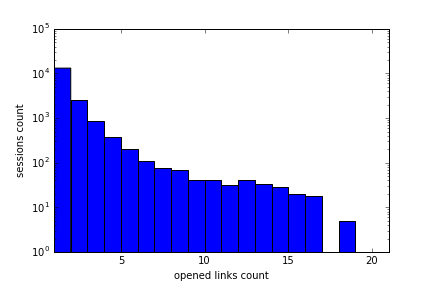
\includegraphics[width=0.5\textwidth]{images/home_page_opened_links_number_hist.png}}
  \hfill
  \subfloat[доли решения]{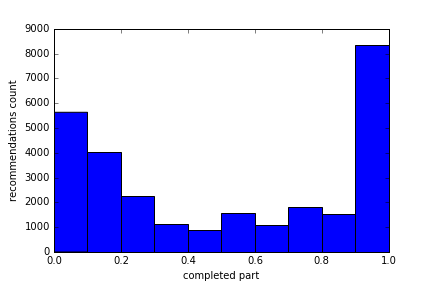
\includegraphics[width=0.5\textwidth]{images/home_page_completed_part_hist.png}}
    \caption{Распределения для простых рекомендаций}
    \label{fig:usual_distibutions}
\end{figure}


\subsection{Контекстные рекомендации}
\indent В случае, если урок, пройденный пользователем, не включен ни в какой курс, то есть не имеет явного следующего за ним урока, пользователю предлагаются рекомендации, сделанные на основе информации о нем и о текущем уроке. В данном случае пользователь наверняка видел рекомендации, что прямо отражается на проценте рекомендательных сессий с реакцией.
\\\indent В таблице \ref{tabular:table_context} также отражены результаты за четыре месяца.

\begin{table}[h]
    \caption{Результаты для контекстных рекомендаций}
    \label{tabular:table_context}
    
    \begin{center}
    \begin{tabular}{ c | r }
      \hline
      Метрика & Значение \\
      \hline	
      \hline
      Число сессий & 26995 \\
      Число сессий с реакцией & 15125 \\
      Процент сессий с реакцией &  56\% \\
      Число открытых рекомендаций (из 5) & 1.48 \\
      Пройденная часть урока & 0.5 \\
      Число отказов от рекомендации & 0 \\
      \hline  
    \end{tabular}
    \end{center}
\end{table}


\\\indent На рис.~\ref{fig:context_distibutions} представлены распределения числа открытых рекомендаций и пройденной части урока.

\begin{figure}[h]
  \centering
  \subfloat[открыто ссылок]{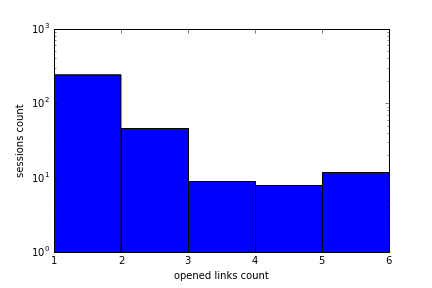
\includegraphics[width=0.5\textwidth]{images/context_opened_links_number_hist.png}}
  \hfill
  \subfloat[доли решения]{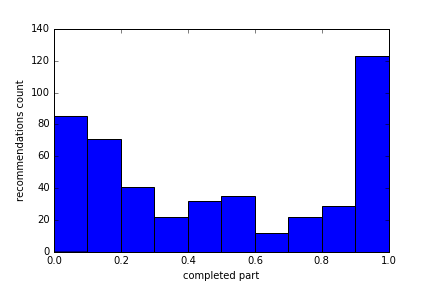
\includegraphics[width=0.5\textwidth]{images/context_completed_part_hist.png}}
    \caption{Распределения для контекстных рекомендаций}
    \label{fig:context_distibutions}
\end{figure}


\section*{Заключение}
\indent В рамках работы была реализована рекомендательная система для образовательного контента, которая теперь используется на платформе \textit{stepic.org}. Эта система совмещает в себе фильтрацию контента и коллаборативную фильтрацию.
\\\indent Структура системы позволяет дополнять ее новыми способами рекомендации, причем значимость каждого способа и его вклад в итоговые рекомендации будет определяться системой автоматически на основе реакции пользователей.
\\\indent Также система предоставляет возможность получать рекомендации в разных ситуациях: как просто при входе на сайт, на домашней странице, так и в процессе обучения, сразу после прохождения урока. 
\\\indent В качестве дальнейших путей развития системы можно указать, во-первых, создание новых правил фильтрации контента исходя из нужд пользователей, во-вторых, совершенствование рекомендательной системы: используя ручную разметку контента можно при рекомендациях использовать изученные и не изученные пользователем темы, предлагать пройти ему что-то, знаний о чем ему не хватает для изучения интересного ему материала. Также возможна работа над проблемой <<холодного старта>>, ситуации, когда про пользователя и про материалы нет достаточного объема накопленных данных, что мешает с уверенностью давать рекомендации.



\setmonofont[Mapping=tex-text]{CMU Typewriter Text}
\bibliographystyle{ugost2008ls}
\bibliography{diploma.bib}


\end{document}
